\section{The Spiritual Regeneration of the World}

Cologero asked me to provide the letter of explanation, despite my reluctance and against my better judgment. I detest any public persona as my work is better accomplished on a different plane of existence. Nevertheless, I am the ultimate authority for Gornahoor, which he operates at my pleasure. Thus, the moment has come to make things clear, not that they haven't been for those able to understand.

Many years ago, Cologero was studying philosophy, particularly thinkers of the Right. He encountered \textbf{Leo Strauss}, whom he read avidly. This meeting of the minds taught him to revere the classical world. It also taught him how to read a philosopher, even those he disagreed with, since, as Nietzsche points out, the false ideas of a great thinker are of more value than the truisms of a mediocre mind. Most importantly, though, he learned to read esoterically. That is, he learned to discern the state of mind of the author behind the text. The text always holds something back and a good author often has sound reasons to leave something for his readers to discern on his own. I encouraged Cologero to apply this way of reading to the medieval thinkers; the results of this sort of analysis are there to see.

Strauss made the interesting point that a great philosopher, or a man who can think things down to their depths, rarely appears. He then claimed that \textbf{Martin Heidegger} was the only philosopher of the 20th century. Needless to say, given Heidegger's well-known sympathy for National Socialism this was rather disconcerting for a Jew to admit. Strauss then made a prediction that engaged Cologero's mind. He speculated that the next great world philosopher might be Asian. That is when Cologero came to me.


\begin{wrapfigure}{rt}{.25\textwidth}
 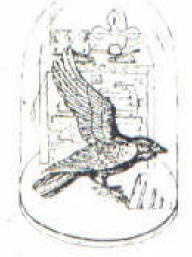
\includegraphics[scale=.5]{a20111116TheSpiritualRegenerationoftheWest-img001.jpg} 
\end{wrapfigure}

His knowledge of Eastern thought was limited to the pop Vedanta all too common among his generation. I led him to authors who were able to bridge Eastern and Western thought, especially \textbf{Sarvepalli Radhakrishnan}, \textbf{Rene Guenon} and \textbf{Ananda Coomsaraswamy}. In particular I asked him to read \textit{The Central Philosophy of Buddhism} by \textbf{T R V Murti} which provides both the material and the mission for Gornahoor. So that it would not remain a mere intellectual task, I encouraged him to take refuge in the Buddha and to practice Tantra and Zen meditation. He then underwent initiation with a Tibetan lama from Boston. I will conclude this with some quotes from Murti; this will make the mission perfectly clear. Our goal is to awaken in some young philosopher the desire to take the \emph{Madhyamika} and apply it to the dominant tradition in the West, just as it had absorbed Greek metaphysics. Evola claimed that Catholicism went only halfway. This move will bring it deeper into the metaphysics of a teaching more ancient and developed than that of the Greeks. First of all, an elite must arise and become conscious of itself. Murti writes:

\begin{quotex}
In the last resort, there must be some considerable body of men who cannot be compelled to behave by external pressure, but who are intrinsically convinced of the worthlessness of material goods. They should have transcended the instinct of possession and must have risen above class and property, like the guardians of state in Plato's Republic. 

\end{quotex}
The West has lost the spiritual unity of Christendom and the results of that loss are plain to see, even among those who remain blind to its cause. It is unlikely to be recovered without the conscious efforts of an elite who can bring in higher spiritual values. Murti makes this suggestion.

\begin{quotex}
Only the spiritual can provide the basis for the society and can be conducive to the realisation of other values. In this regard, Mahayana absolutism and the Advaita Vedanta are valuable as providing the basis on which a world-culture can be built. It is only absolutism that can make for the fundamental unity of existence and at the same time allow differences. … The Vedanta is traditional in outlook and is bound to the authority of the Veda and perhaps it presupposes a specific milieu in which alone it can thrive. The Mahayana is quite liberal and it has proved its capacity to accommodate itself to various religious and social structures, to revitalise and absorb them.

\end{quotex}
Unfortunately, this is all too easily misunderstood as a call to take on the outer trappings of Buddhism rather than the spiritual regeneration it is encouraging. The net effect is not spiritual unity, but a further division, as Westerners then come to loathe their own Sacred Tradition. They create Strife rather than Love, as your \textbf{Empedocles} put it. Murti then offers some quotes from Radhakrishan, but what he writes about Guenon is more pertinent to Gornahoor readers.

\begin{quotex}
To take an example for the West, M. Guenon has made a commendable effort to interpret the true spirit of Hindu culture to the West in his many works. \emph{The form of regeneration consists, for M. Guenon, not in a fusion of synthesis of the two cultures, but in the West regaining, as the result of a dynamic turn in its present trend, those springs of true spirituality through the help of the East.} It would be hazardous to forecast the time of the change or the precise manner in which it would be brought about.

\end{quotex}
But we can specify the general manner. It will not be from a philosophy of the academic type that everyone will miraculously accept. No, there must be a gnosis, an experiential knowing, that transcends words and thoughts. This the Madhyamika makes clear: it is not a matter of debate, dialectics or persuasion. That is why Cologero emphasizes the spiritual exercises so much. Spiritual unity will come, as he points out, from the depths, not from superficial and merely verbal agreement. Murti explains:

\begin{quotex}
What we need is the realisation of the spiritual which is the bedrock of all our endeavour. Only mystical religion, which eminently combines the unity of Ultimate Being with the freedom of different paths for realising it, can hope to unite the world. The student of philosophy can only suggest that the Madhyamika Absolutism can serve as the basis for a possible world culture. It is not his province to show how best this could be implemented, what practical shape this would assume and at which point and time in the affairs of the world this could be introduced. These are questions which the religious reformer might answer, and even he has to depend upon the spiritual guidance and direction from above.

\end{quotex}
Murti concludes with a warning against scholars and professors, although he himself is one. The regeneration won't come from them as even Murti is too irenic and sanguine. He writes:

\begin{quotex}
We must end with a note of warning. It is possible, in our enthusiasm, to overrate the part played by scholarship and the theoretical understanding of things in the task of regeneration. It is good to remember that history does not record of a single instance of a spiritual revolution of global dimensions brought out by a band of scholars or skillful thinkers. The malady of the world is far too universal and deep-seated for remedies to be prescribed direct from books. A spiritual genius of the order of \textbf{Buddha} or \textbf{Christ} alone knows how to strike at the thing. But even a theoretic understanding of the Madhyamika absolutism should prove of value by way of preparing the background for the \emph{spiritual regeneration of the world}.

\end{quotex}
No, it is the man of vision, the man of action, who understands and engages in the greater and lesser battles who will bring it about. The world is not awaiting a new theory, since there is nothing new under the sun. By overemphasizing unity, Murti betrays his own theory. There is neither unity nor conflict, there is both unity and conflict, there is no unity but there is conflict, there is unity but no conflict: this cannot be resolved by thought alone, but rather by action, that is, bringing the potential into act, non-being into being, making the unreal, real. Ideas have no existence on their own, but take on life in the mind of a conscious being. So we await not a new system, but a man, or rather the coming of a man-god. Only a god can save you now.



\flrightit{Posted on 2011-11-16 by Losang Shenphen }

\begin{center}* * *\end{center}

\begin{footnotesize}\begin{sffamily}



\texttt{charlotte on 2011-11-17 at 12:18 said: }

I think you are right, by the way, to emphasise the need for action – we need to be the change we want to see. After many years of meditation, soul searching and climbing the holy mountain I realised there was simply nothing else for it but to climb back down and actually DO something. I still believe in the power of prayer of course, but the need to help others and to actually make sommething of the earth is fundamental to the spiritual mission of those who `know better', so to speak. However when I recently exhorted some `colleagues' in this field to do the same I was met with a very unfriendly response, despite the fact that the key text they work with (Meditations on the Tarot) explicitly says we must do this, that the last great test of the spiritual seeker is to walk the humble road of work made into love, rather than disappearing up the mountain and floating off on a sacred cloud for the good of no-one but self. The most spiritual person I know is a man who would feels he lacks intelligence compared to me and others who've been `educated', but I'm in awe in his presence, he works and gives for all he's worth and is known to all around him by his fruits, he is the archetypal hero and man of action. (yes I love him, lol :-)) Jesus Christ was a man who showed the way by action in the ultimate sense – and yes, I love him too, He truly is the source of all love in this creation and we find love by expanding ourselves towards Him, away from the saturated ego. Disolution, they say, is the secret of the great work – disolving in the sea of love…


\hfill

\texttt{charlotte on 2011-11-17 at 12:18 said: }

I think you are right, by the way, to emphasise the need for action – we need to be the change we want to see. After many years of meditation, soul searching and climbing the holy mountain I realised there was simply nothing else for it but to climb back down and actually DO something. I still believe in the power of prayer of course, but the need to help others and to actually make sommething of the earth is fundamental to the spiritual mission of those who `know better', so to speak. However when I recently exhorted some `colleagues' in this field to do the same I was met with a very unfriendly response, despite the fact that the key text they work with (Meditations on the Tarot) explicitly says we must do this, that the last great test of the spiritual seeker is to walk the humble road of work made into love, rather than disappearing up the mountain and floating off on a sacred cloud for the good of no-one but self. The most spiritual person I know is a man who would feels he lacks intelligence compared to me and others who've been `educated', but I'm in awe in his presence, he works and gives for all he's worth and is known to all around him by his fruits, he is the archetypal hero and man of action. (yes I love him, lol :-)) Jesus Christ was a man who showed the way by action in the ultimate sense – and yes, I love him too, He truly is the source of all love in this creation and we find love by expanding ourselves towards Him, away from the saturated ego. Disolution, they say, is the secret of the great work – disolving in the sea of love…


\hfill

\texttt{Jupiter on 2011-11-17 at 13:18 said: }

You know, before this article, I had quite a bit of respect for this site. For the most part this place has avoided some of the more bizarre and theosophically-oriented problems that a lot of other so-called ``Traditionalist" communities and publications succumb to.

Until now.

Stick to Tradition and leave the traditionalist claptrap out of it. Let's hear more Plotinus, St. Antony, Adi Shankara, Shakyamuni Buddha, and Lao Tzu and less Gurdjieff and Schuon madness or talk of who is behind what. Nobody who is attracted to this sort of place cares…That sort of bullshit is for the rest of Kali Yuga. We're here, reading what we read, because we're trying to escape the exact sort of dialectical wankery that Gornahoor's been spitting out as of late.


\hfill

\texttt{Gabe Ruth on 2011-11-17 at 14:53 said: }

Thank you for that summary, I found it quite stirring. 

To the haters: you can get cargo-cult traditionalism and therapeutic spiritualism from a lot of places if you like. I appreciate people who believe what they say, seek to live it, and try to share their methods and experiences to the extent it is possible in this medium.


\hfill

\texttt{Graham on 2011-11-17 at 14:54 said: }

Losang,

Thank you for the letter of explanation. What, however, is the goal? Are you now to take a more open role? What was the purpose for hiding yourself in the first place? Most importantly, as EXIT asked, who are you? Revealing yourself as the authority behind Gornahoor raises more questions than it answers.

Forgive me for that barrage. Having followed this site for some two-odd years it's a surprise to learn that the man I thought was behind it isn't really. Or is he…? Could you explain your relationship with the site in a bit more detail? Do you set the agenda? I'm always interested in `wheels behind wheels' but you'll forgive me if I say it feels somewhat Masonic. It is after all concerning to learn that what one took to be an move to tradition of a mostly Western provenance in fact has an Easterner `pulling the strings', even if we suppose he's of good will.

I notice with interest that you didn't include Evola in your reading list, while you did include Guenon and Coomaraswamy. Is that an oversight or something more pointed?

Graham


\hfill

\texttt{EXIT on 2011-11-17 at 16:41 said: }

[ Response from Cologero:

As someone who reads Gornahoor assiduously, you have a remarkable ability to understand nothing.

1) Where is the post where Gornahoor has proclaimed the ``one and only truth"?

2) Where and when have you ever offered a specific criticism rather than vague inanities?

3) Where have we shown a ``sentimental" attachment to Christianity? No, we have convincingly demonstrated that a specific era of Western history was characterized by a traditional social structure and understood a gnosis beyond rational thought.

That is an objective, not a sentimental, judgment. The paradox is that non-Christians recognize it, yet contemporary Christians seem rather embarrassed.

4) An attachment to a paganism that never existed anywhere is more properly described as ``sentimental". That is why those with the mentality of a shudra imagine themselves to be great gods and Nietzschean supermen, and go seeking after runes. Question to readers: Why did even Leif Ericson reject this?

5) You need no one, EXIT? So you are indeed a self-initiator. You are the wishful thinker. If you have misunderstood us, perhaps even some more intelligent readers have. Have we not written of the ``one and only guru transmigrant, etc)"? Have you not understand that it is a call for you to be that god-man? or a great prince, warrior, priest, philosopher or artist? That is the waiting … an intelligent man knows how to wait.

If we continue to get such dullards reading Gornahoor … it may be time to wait for a new generation to appear.

]

L.S.: ``you flatter us by thinking we are the ones who are closest to the ``one and only truth"."

Acting as if one had the one and only truth is not the same thing as believing it, for there is no ``one and only" truth. Criticisms are therefore valid even though they may go against something which you hold a sentimental attachment to, such as Christianity.

As for a god-man who is going to come and save us all, that is just wishful thinking, something that I despise, for it implies dualism. I wait for no one. I need no one. And surely don't look for anyone for ``salvation".


\hfill

\texttt{charlotte on 2011-11-17 at 17:14 said: }

\url{http://alchemical-weddings.com/alchemical-weddings/pros-theon}


\hfill

\texttt{Graham on 2011-11-18 at 09:58 said: }

Logres,

I agree, and Gornahoor has been fruitful indeed. If Losang Shenphen is behind it then we have every reason to judge well of him. Still, after following the site and even its programme for some time I feel invested in it, and therefore somewhat surprised, possessive, and suspicious when I realize it isn't quite what I thought it was. Asking questions and being less than completely equanimious is a fair reaction. But do Losang and Cologero owe us answers? Not at all. I am patient enough to watch things develop at their own pace.

Graham


\hfill

\texttt{Logres on 2011-11-19 at 00:26 said: }

Graham, thanks for your comment, \& of course I too am intrigued \& interested in learning more. Certainly, question here is one of authenticity – it comes up in ecclesiastical circles regarding ordination and succession. Often times, in difficult spots, it becomes disputed and unclear. In such times, I think that it is always good to suspend judgement, and look to the aim and result, rather than the standard, since it is precisely the standard which is already compromised. I would personally be willing to accept almost any level of aid to the West spiritually, provided the tendency was to establish the West's capability of self-governance. Since, at some level, the common origin must obtain and persist, it is our duty to expect exactly this sort of help, and to endeavor to respond to it. I agree it requires a certain spiritual gift of discernment.


\hfill

\texttt{Boreas on 2011-11-19 at 03:55 said: }

Thanks for this clarification – or apparent confusion, as it seems to be – about the motivations, purposes and personalities behind Gornahoor. There are visible authorities \& leaders and invisible authorities \& leaders, and everything we see around us is the result of both of these. The only thing that matters is the nature of both of these, and thus far Gornahoor and its (visible) contributors have been non-partisan, informative, enlightening and objective in their work.

Thus, I see no problem here. Things would be different if people were being led to something the nature of which remains completely unknown to them, or if people were being pressured to some partial goal / direction out of fear etc.

Become who you are.


\hfill

\texttt{Chmitt on 2011-11-19 at 05:25 said: }

The image in this post is drawn from \url{http://www.tanmanho.com/}.

I'm beginning to suspect that Cologero is actually the man in the photo shown on that website, and based in Malaysia. It seems that this benevolent Oriental has extended help to us floundering westerners in the guise of everyone's favorite Italian uncle.

Greetings, Cologero – or rather, Professor Sir Dr. Tan Man-Ho Cologero!


\hfill

\texttt{charlotte on 2011-11-19 at 13:39 said: }

regarding `sentimental attachments' to Christianity, the muslim president of America would be proud of your disdain for love's greatest passion.

What a joke to see the fuss about Iran, Obama's secret friend….or maybe I got it wrong, maybe north Africa hasn't recently been handed over to radical Muslim brotherhoods like Al Qaeda, maybe the US president didn't really arrive on a white horse in the – colorado was it? – stadium?

conversion to Islam sounds pretty good from an intellectual point of view – heck, I love Rumi, Gibran, Hafiz etc, I really do – but shall we just take a look at the human rights issues, seriously, shall we just have a think about the socio-political reality it would entail? Wouldn't all be hookah pipes and philosophical chit chat in the tea rooms, THAT I can tell you. Bring out the bullwhips, the women are thinking….


\hfill

\texttt{francismercuri on 2015-11-10 at 22:43 said: }

How quickly humans turn on one another; some of these comments seem to just be looking for confrontation for its own sake.

In posts going back quite some time, Gornahoor stated that when the 1001 post goal neared, that the project would make clear what the purpose had been the whole time–the above is not an off-the-cuff twist, or ``change" in direction–it was present the entire duration, and the supra entry had been planned long ago.

Current detractors should observe that the above entry notes:

``That is, he learned to discerne the state of mind of the author behind the text. The text always holds something back and a good author often has sound reasons to leave something for his readers to discern on his own". 

Who ``is" Losang Shenphen? Is he a ``real" individuality apart from Cologero, or is he a sort of pseudopigraphal whimsy? Who cares and why ought it matter? What matters involves nothing but the totality of the Gornahoor posts, and their ultimate grounding in the trajectories noted above.

Then, ``Nevertheless, I am the ultimate authority for Gornahoor, which he operates at my pleasure".

Why ought anybody assume that this statement refers to a ``site" and some factual administration? Isn't ``Gornahoor", after all, something preceding net technology?


\hfill

\texttt{White Rabbit on 2015-11-11 at 03:07 said: }

Gornahoor is a three-brained extraterrestrial being (maybe an Exonordic alien) from the planet Saturn, while Losang is just some boring oriental weirdo. The thing that I find most interesting here is the ``sort of analysis" mentioned. Reading the medieval thinkers that way could illuminate the face of our past.


\hfill

\texttt{Sparrow on 2015-11-12 at 13:43 said: }

@ White Rabbit,

It seems rather silly to use ``Oriental," negatively, when those cultures are largely the sources for Guenon and Evola, without neither of whom we would not have this illuminating site.


\hfill

\texttt{White Rabbit on 2015-11-13 at 18:47 said: }

It is – I was attempting humor (now maybe I should clarify that I agree with Mr. Mecuri's comment).


\hfill

\texttt{THAT on 2017-06-07 at 06:46 said: }

«Our goal is to awaken in some young philosopher the desire to take the Madhyamika and apply it to the dominant tradition in the West, just as it had absorbed Greek metaphysics.»

It would be interesting to learn more about this possibility from Gornahoor's perspective. I searched the archive, but there are exceedingly few posts that barely touch upon the subject at all. If the goal has been to seed such a daring and pioneering venture as applying Madhyamika to the Tradition of the West, one might expect the theme to have appeared more prominently throughout the posting history of this blog.


\hfill

\texttt{Cologero on 2017-06-12 at 08:14 said: }

@Tat Tvam Asi

Madhyamika is implicit throughout.


\hfill


\end{sffamily}\end{footnotesize}
